\subsection{La base de données}

On choisi de travailler sur la base de données Kaggle \href{https://www.kaggle.com/competitions/leaf-classification}{Leaf Classification} (Classification de feuilles). Cette base de données présente l'avantage d'avoir déjà été nettoyée pour être utilisée.\\

Cette base de données a extrait 3 caractéristiques d'images de feuilles, à savoir la description de leur forme, un histogramme de leur texture, et un histogramme de leurs marges. Ces trois caractéristiques sont représentées par des vecteurs à 64 dimensions. On a donc un total de \bf{192 caractéristiques}.\\

Le but est d'associer chaque feuille à l'une des \bf{99 espèces}. On dispose pour cela de 16 exemples par catégorie, pour un total de \bf{1 584 échantillons}.\\

La base de données est de plus séparée en deux jeux de données : un jeu d'entraînement supervisé de \bf{990 échantillons} (10 de chaque espèce, voir \autoref{fig:species_repartition}) et un jeu de test non supervisé de \bf{594 échantillons} (6 de chaque espèce).

\begin{figure}[h]
    \centering
    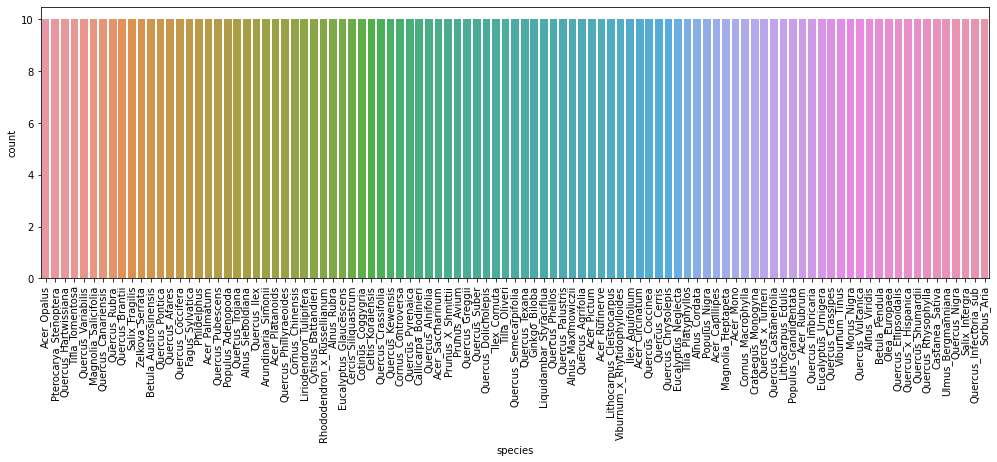
\includegraphics[scale=0.48]{Images/graphiques/species_repartition.png}
    \caption{\it{Répartition des espèces dans le jeu d'entraînement}}
    \label{fig:species_repartition}
\end{figure}